\documentclass[12pt,a4paper]{article}

\usepackage[margin=1in]{geometry}
\usepackage{graphicx}
\usepackage{longtable}
\usepackage[dutch]{babel}
\usepackage{url}
\usepackage{caption}
\usepackage{amsfonts}

\usepackage[section]{placeins}

\usepackage{color}

\usepackage{xypic}
\usepackage[all,color]{xy}
\xyoption{all}

\usepackage{fancyhdr}
\pagestyle{fancy}
\fancyhead{}
\fancyfoot{}
\renewcommand{\headrulewidth}{0mm}
\rfoot{\thepage}    
\cfoot{}
\lfoot{Practicum Numerieke Wiskunde - Christophe Van Ginneken}


\geometry{a4paper}

\title{\vspace{-6ex}Practicum Numerieke Wiskunde\vspace{-1.5ex}}
\author{Christophe Van Ginneken}
\date{\vspace{-1.5ex}\today}

\begin{document}
\maketitle
\vspace{-2cm}
\section{Inleiding}

We zoeken in dit practicum de maxima van een intensiteitspatroon voor een \'e\'en-spleet-diffractie. Deze wordt gegeven door
\begin{equation} \label{eq:intensitypattern}
I(\theta) = I_{max} \frac{\sin^2 \alpha}{\alpha^2},
\end{equation}
met
\begin{equation} \label{eq:alpha}
\alpha = \frac{\pi \ a \ \sin \theta}{\lambda}.
\end{equation}
In deze vergelijking is $a$ de breedte van de spleet waardoor het licht met golflengte $\lambda$ op een scherm valt. De verhouding tussen $a$ en $\lambda$ is typerend voor de manier waarop dit licht op het scherm valt. Indien deze verhouding groter is dan 1, zal er interferentie optreden. We kunnen deze verhouding dus schrijven als
\begin{equation} \label{eq:a/lambda}
r=\frac{a}{\lambda}.
\end{equation}
Hierdoor kan vergelijking (\ref{eq:alpha}) geschreven worden als
\begin{equation} \label{eq:alpha-simple}
\alpha = r \pi \ \sin\theta
\end{equation}
en kunnen we vergelijking (\ref{eq:intensitypattern}) voluit schrijven als
\begin{equation} \label{eq:intensitypattern-full}
I(\theta) = I_{max} \left(\frac{\sin(r \pi \ \sin \theta)}{r \pi \ \sin \theta}\right)^2.
\end{equation}
$I_{max}$ is een maat voor de maximale intensiteit van de projectie op het scherm. Figuur \ref{fig:single-slit-diffraction-components} toont een concreet voorbeeld met alle aspecten van het intensiteitspatroon en hun aandeel in het uiteindelijk geprojecteerde diffractiepatroon. In dit voorbeeld is $I_{max} = 2$ en is tevens de waarde van het extremum van de functie voor $\theta = 0$. Verder is de waarde van de verhouding tussen de grootte van de spleet en de golflengte $r=3$, wat zich vertaalt in drie (positieve) maxima.

We zullen aantonen dat de maxima van $I(\theta)$ bereikt worden wanneer $\alpha$ een wortel is van de niet-lineaire vergelijking
\begin{equation} \label{eq:non-linear}
\tan\alpha - \alpha = 0.
\end{equation}
Vervolgens zullen we door middel van vier kandidaat substitutiemethodes trachten deze nulpunten te benaderen.

\begin{figure}[h]
\begin{center}
 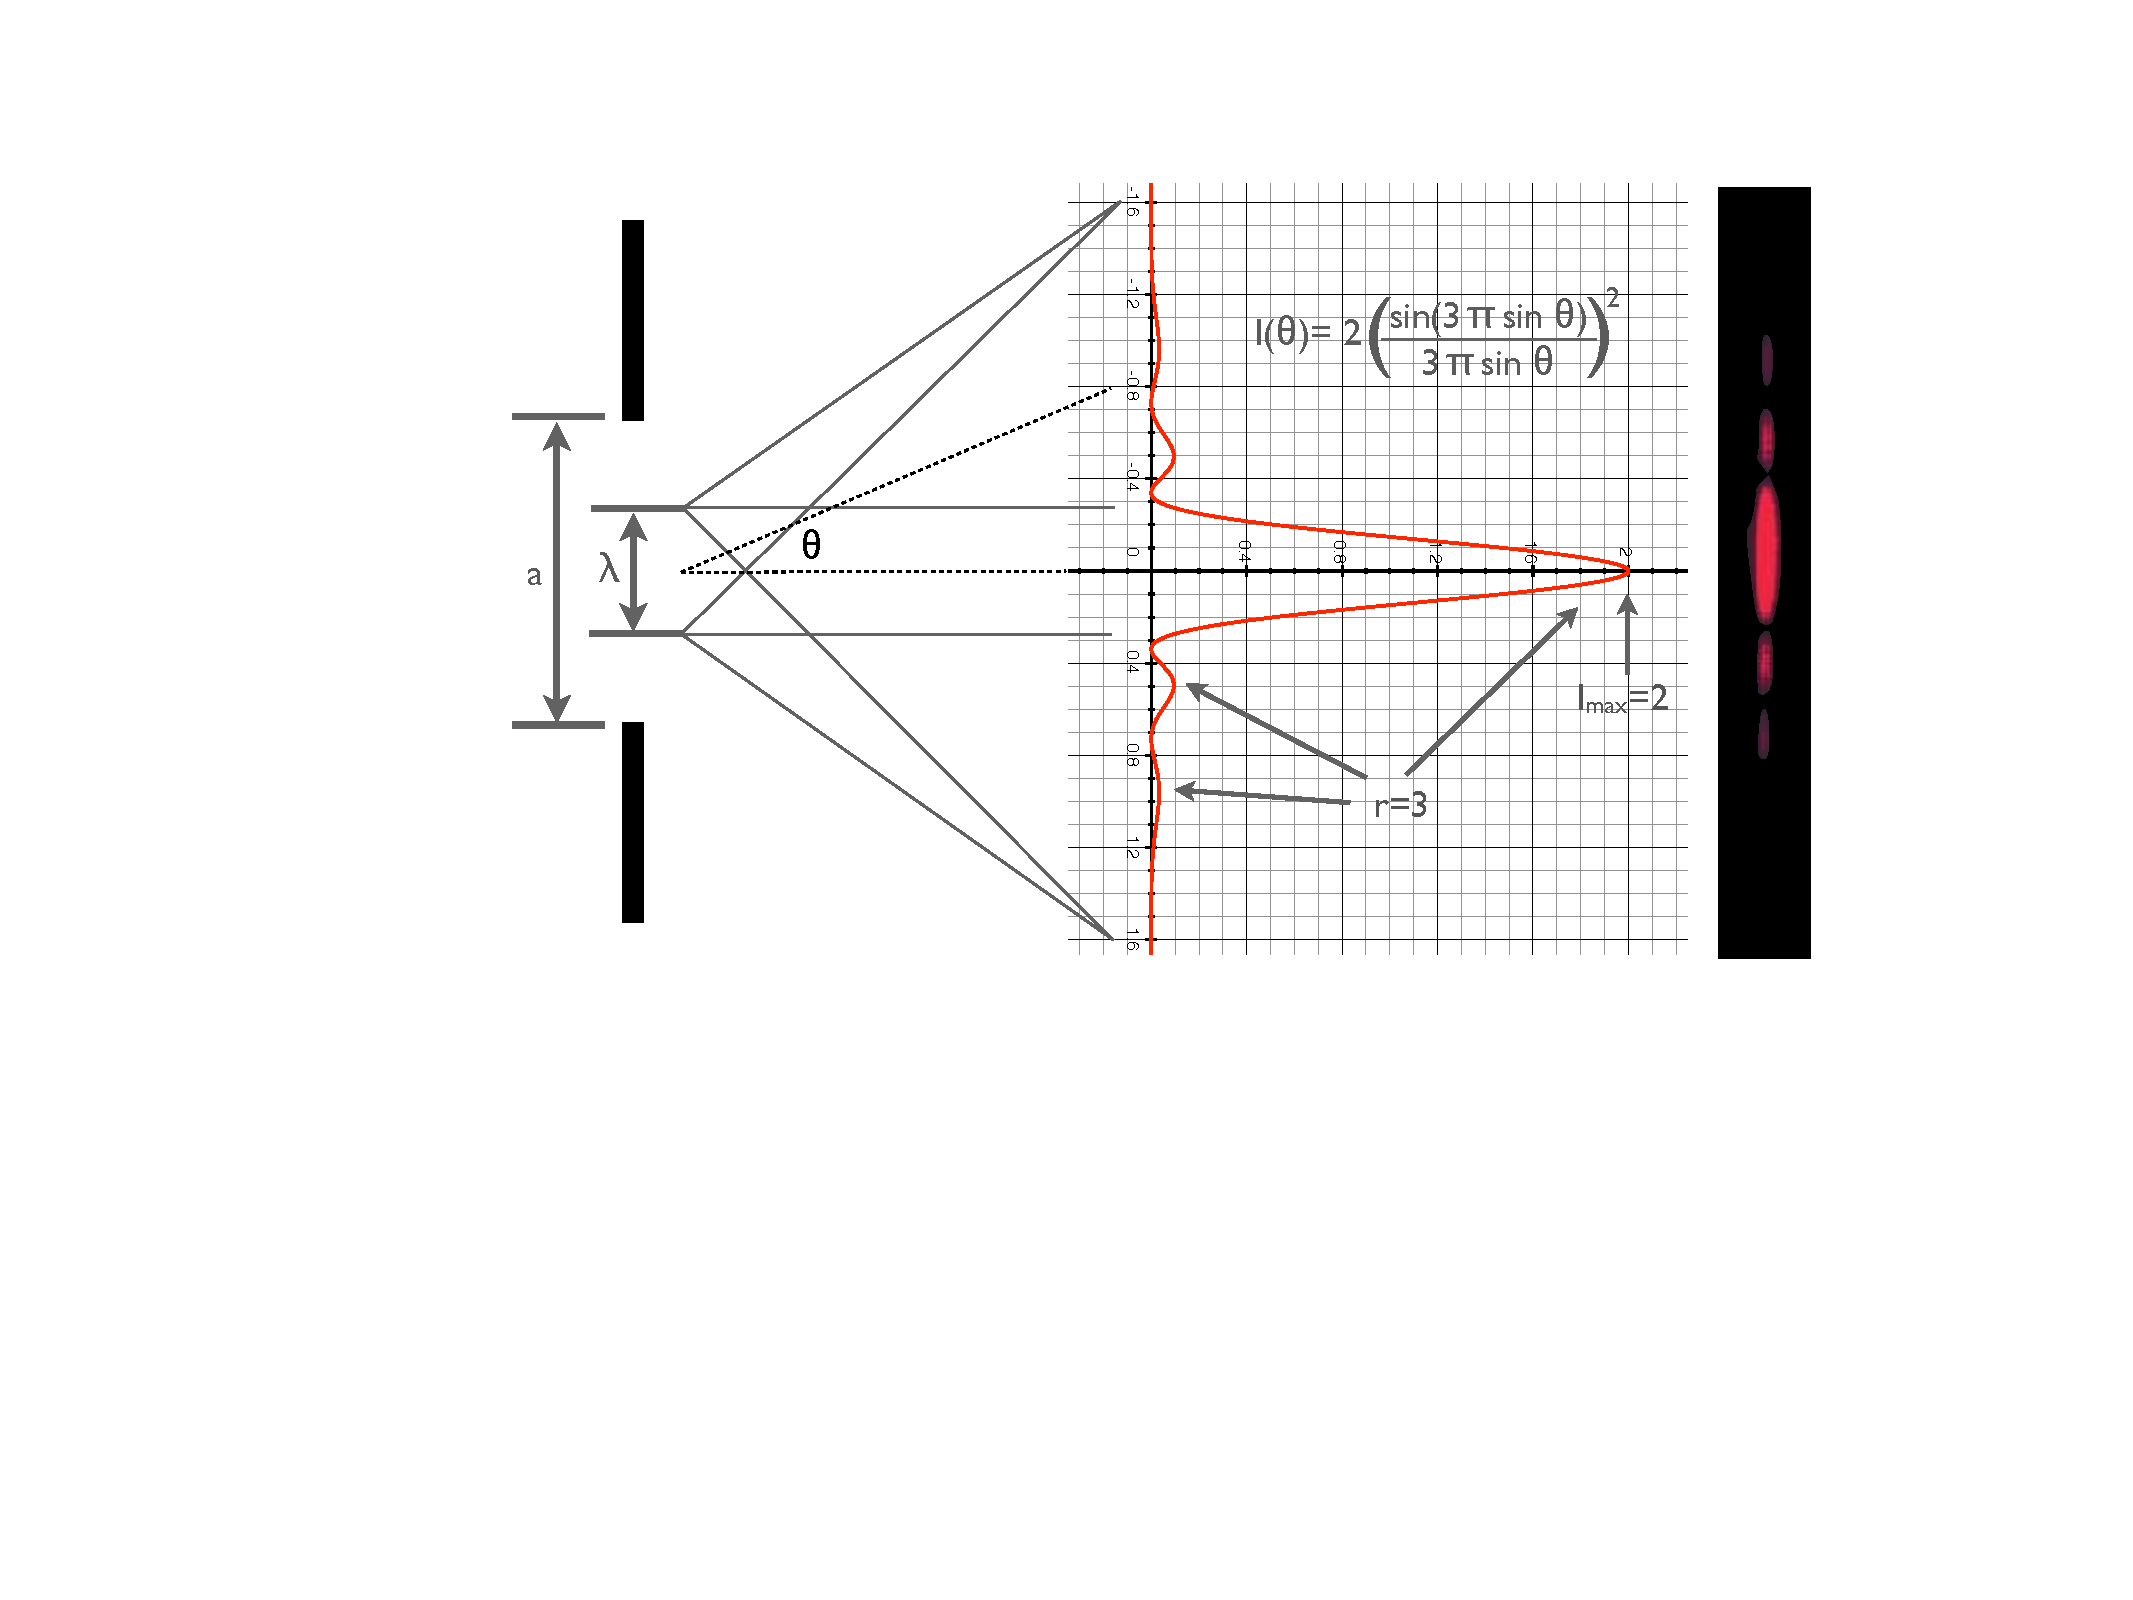
\includegraphics[width=110mm]{resources/single-slit-diffraction-components.pdf}
 \caption{Componenten van een \'e\'en-spleet-diffractie}
  \label{fig:single-slit-diffraction-components}
\end{center}
\end{figure}

\subsection{Equivalentie maxima van de niet-lineaire vergelijking}

De minima en maxima van een functie kunnen gevonden worden door het bepalen van de nulpunten van de afgeleide van die functie. Figuur \ref{fig:maxima} toont een voorbeeld van een intensiteitspatroon ($I_{max}=2, r=3$) en de bijhorende afgeleide. We zien dat de nulpunten van de afgeleide functie overeenkomen met de minima en maxima van het intensiteitspatroon.

\begin{figure}
\begin{center}
 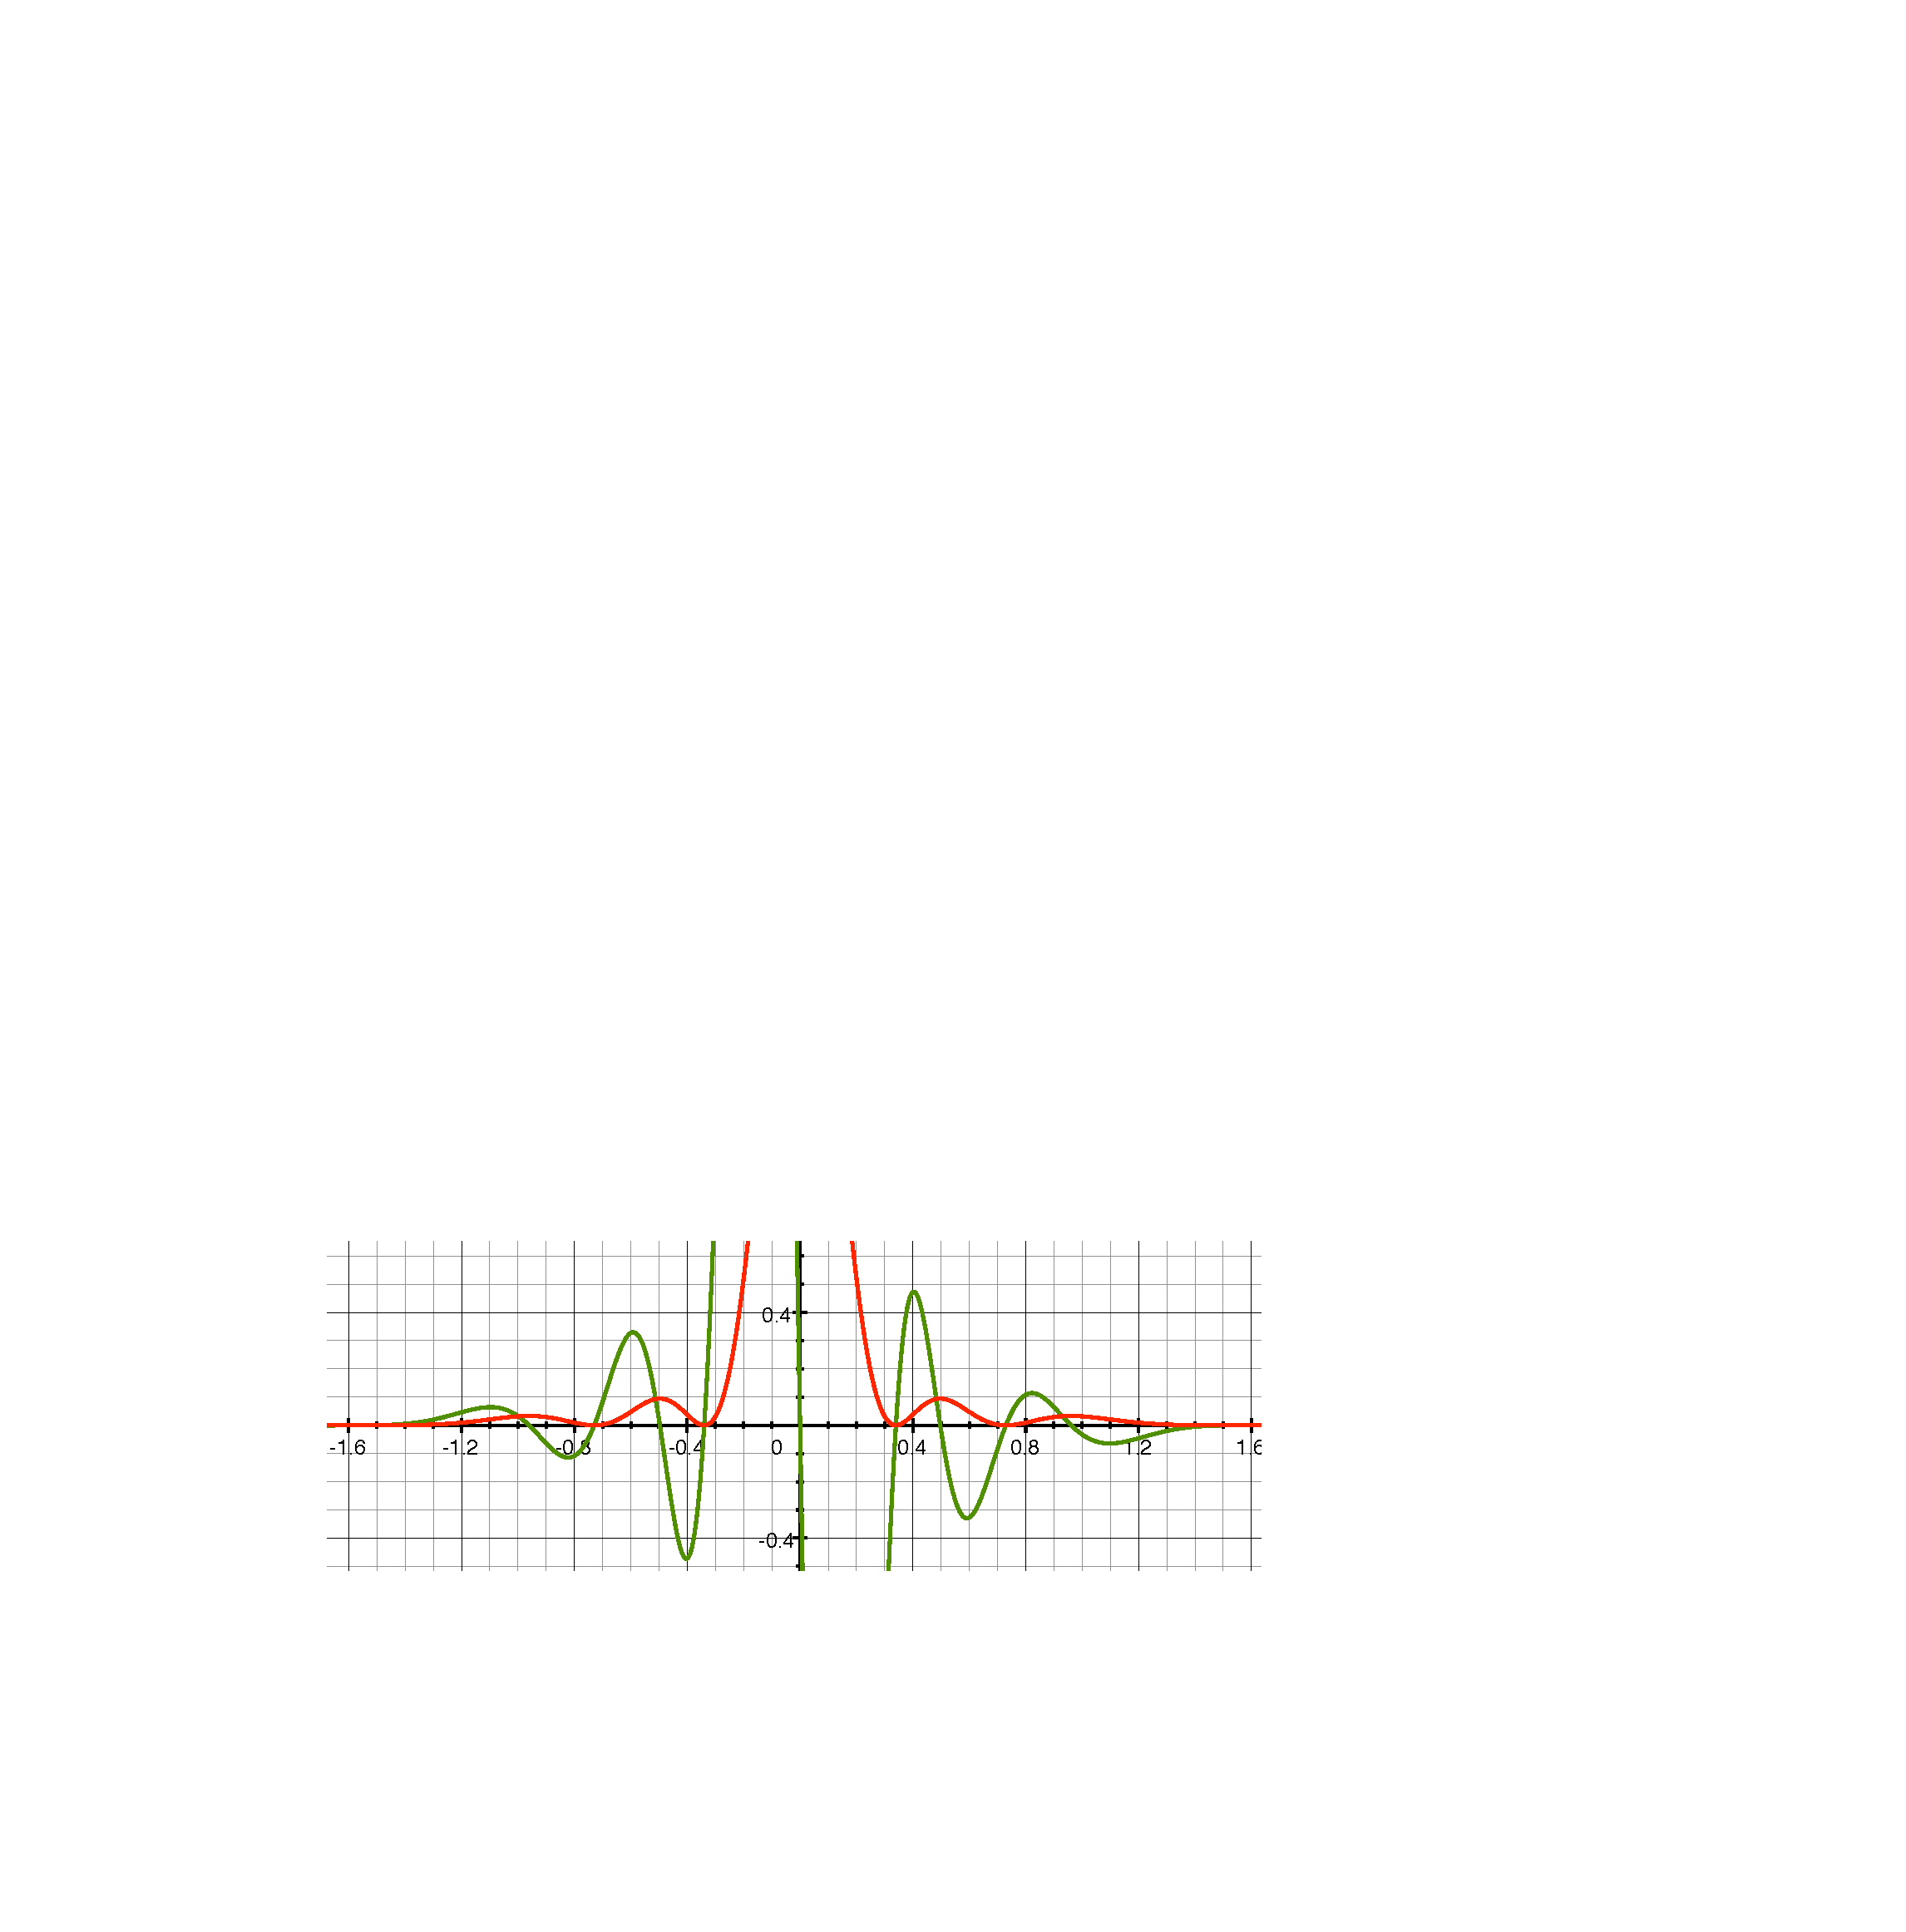
\includegraphics[width=100mm]{resources/maxima.pdf}
 \caption{Intensiteitspatroon (rood) en overeenkomstige afgeleide functie (groen)}
  \label{fig:maxima}
\end{center}
\end{figure}

We vertrekken dus van de afgeleide van vergelijking (\ref{eq:intensitypattern-full}). 

\begin{equation} \label{eq:derivate}
2 \ . \frac{\sin( r \pi \ \sin \theta)}{r \pi \ \sin \theta} \ . \ \frac{\cos(r \pi \ \sin \theta)\ . \ r \pi \ \cos \theta \ . \ r \pi \ \sin \theta - \sin(r \pi \ \sin \theta) \ . \ r \pi \ \cos \theta}{(r \pi \ \sin \theta)^2}
\end{equation}

Hierbij laten we de factor $I_{max}$ buiten beschouwing. Deze is slechts een multiplicator en bepaalt de \emph{hoogte} van het extremum. Vergelijking (\ref{eq:derivate}) kan vereenvoudigd worden tot

\begin{equation} \label{eq:derivate-simple}
\frac{2 \ . \ \sin( r \pi \ \sin \theta) \ . \ \cos \theta \ . \ ( r \pi \ \sin \theta \ . \ \cos( r \pi \ \sin \theta) - \sin( r \pi \ \sin \theta))}{r^2 \pi^2 \ \sin^3 \theta}
\end{equation}

De teller van vergelijking (\ref{eq:derivate-simple}) bevat drie factoren die aanleiding kunnen geven tot nulpunten: $\sin( r \pi \ \sin \theta)$, $\cos\theta$ en $r \pi \ \sin \theta \ . \ \cos( r \pi \ \sin \theta) - \sin( r \pi \ \sin \theta)$.

$\cos\theta$ zal nulpunten opleveren voor $\theta = \frac{1}{2} \pi (4n-1), n \in \mathbb{Z}$. Concreet zijn dit bijvoorbeeld $-\frac{\pi}{2}$ en $\frac{\pi}{2}$. We zien in figuur \ref{fig:cosine-period} dat dit overeenkomt met de punten waar twee opeenvolgende iteraties van de functie van het patroon aan elkaar sluiten. De periodiciteit van de $\cos$-functie bepaalt op die manier de periodiciteit van de diffractie-functie.

\begin{figure}
\begin{center}
 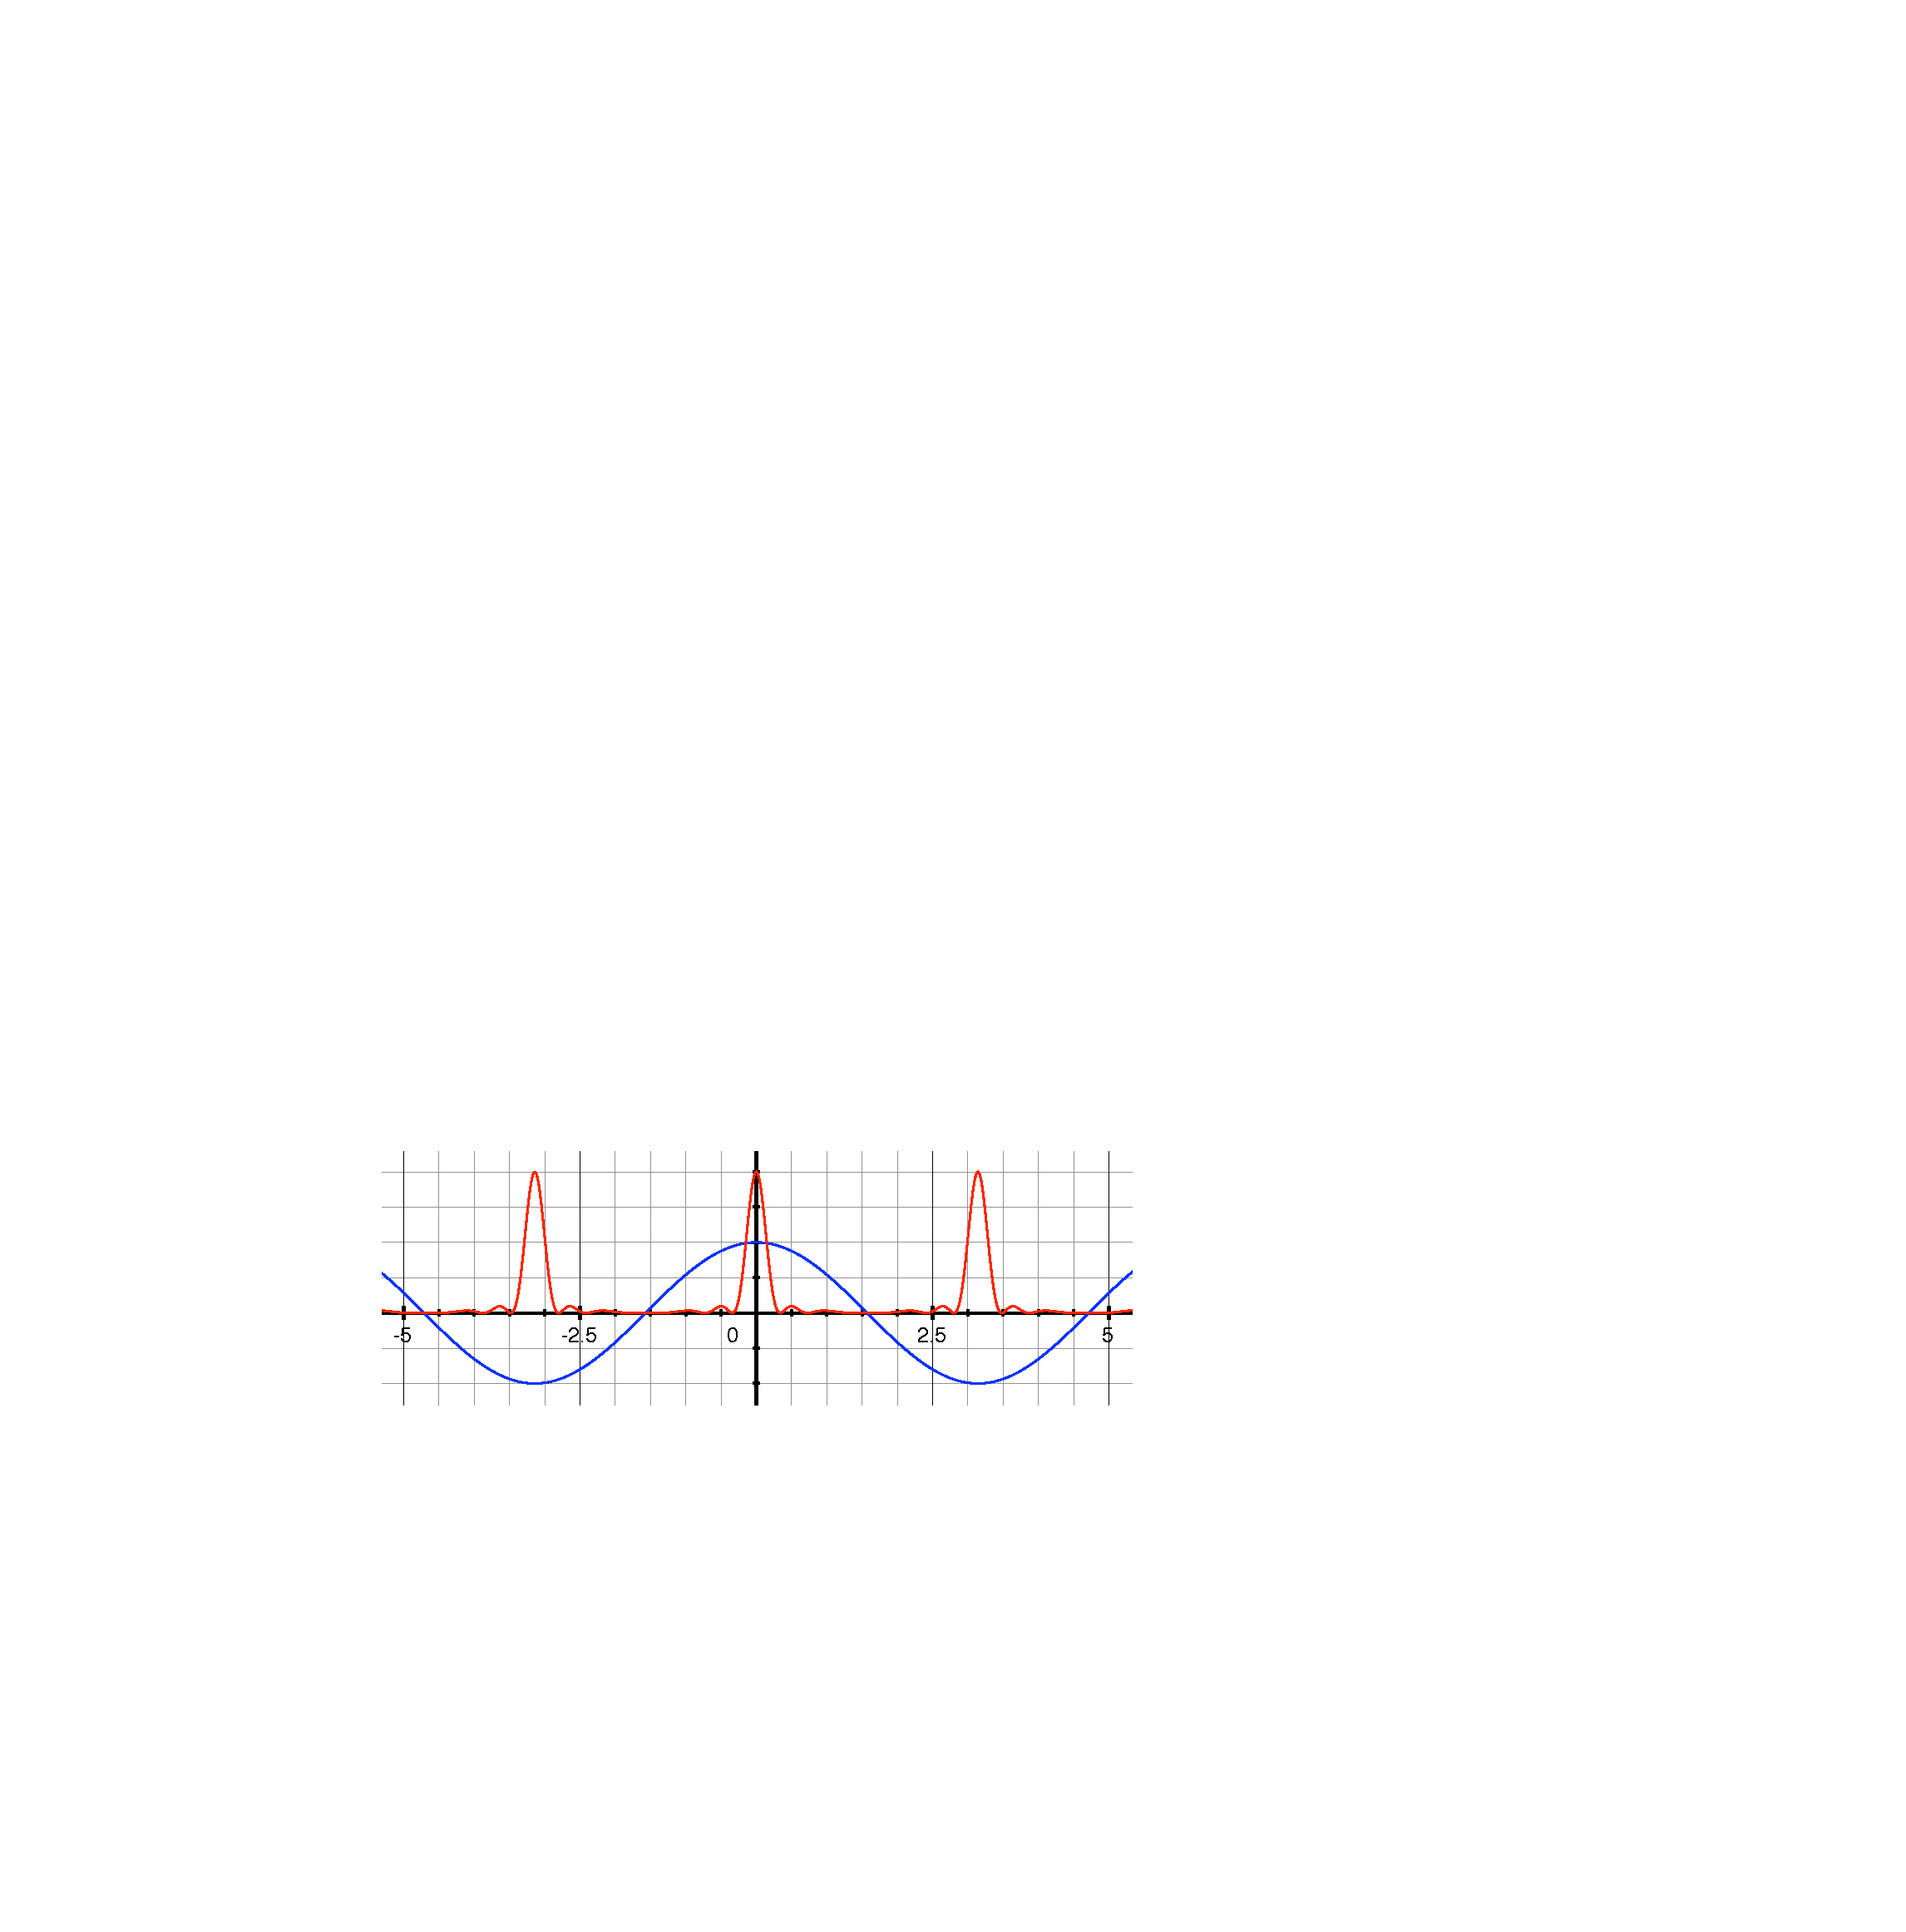
\includegraphics[width=100mm]{resources/cosine-period.pdf}
 \caption{Periode van de $\cos$-functie}
  \label{fig:cosine-period}
\end{center}
\end{figure}

We weten dat $\sin\theta$ nulpunten oplevert voor $\theta = n \pi, n \in \mathbb{Z}$ en dus ook als $r \pi \ \sin\theta = n \pi$ of als $\sin \theta = \frac{n}{r}$. In ons voorbeeld is $r=3$ en zijn de waarden van $\theta$ voor $n = 1, 2$ gelijk aan $sin^{-1} \frac{1}{3} = 0.3398$ en $sin^{-1} \frac{2}{3} = 0.7297$. Dit zijn telkens minima. Figuur \ref{fig:minima} toont dat de sinus-factor van de afgeleide zorgt voor de minima van het intensiteitspatroon.

\begin{figure}
\begin{center}
 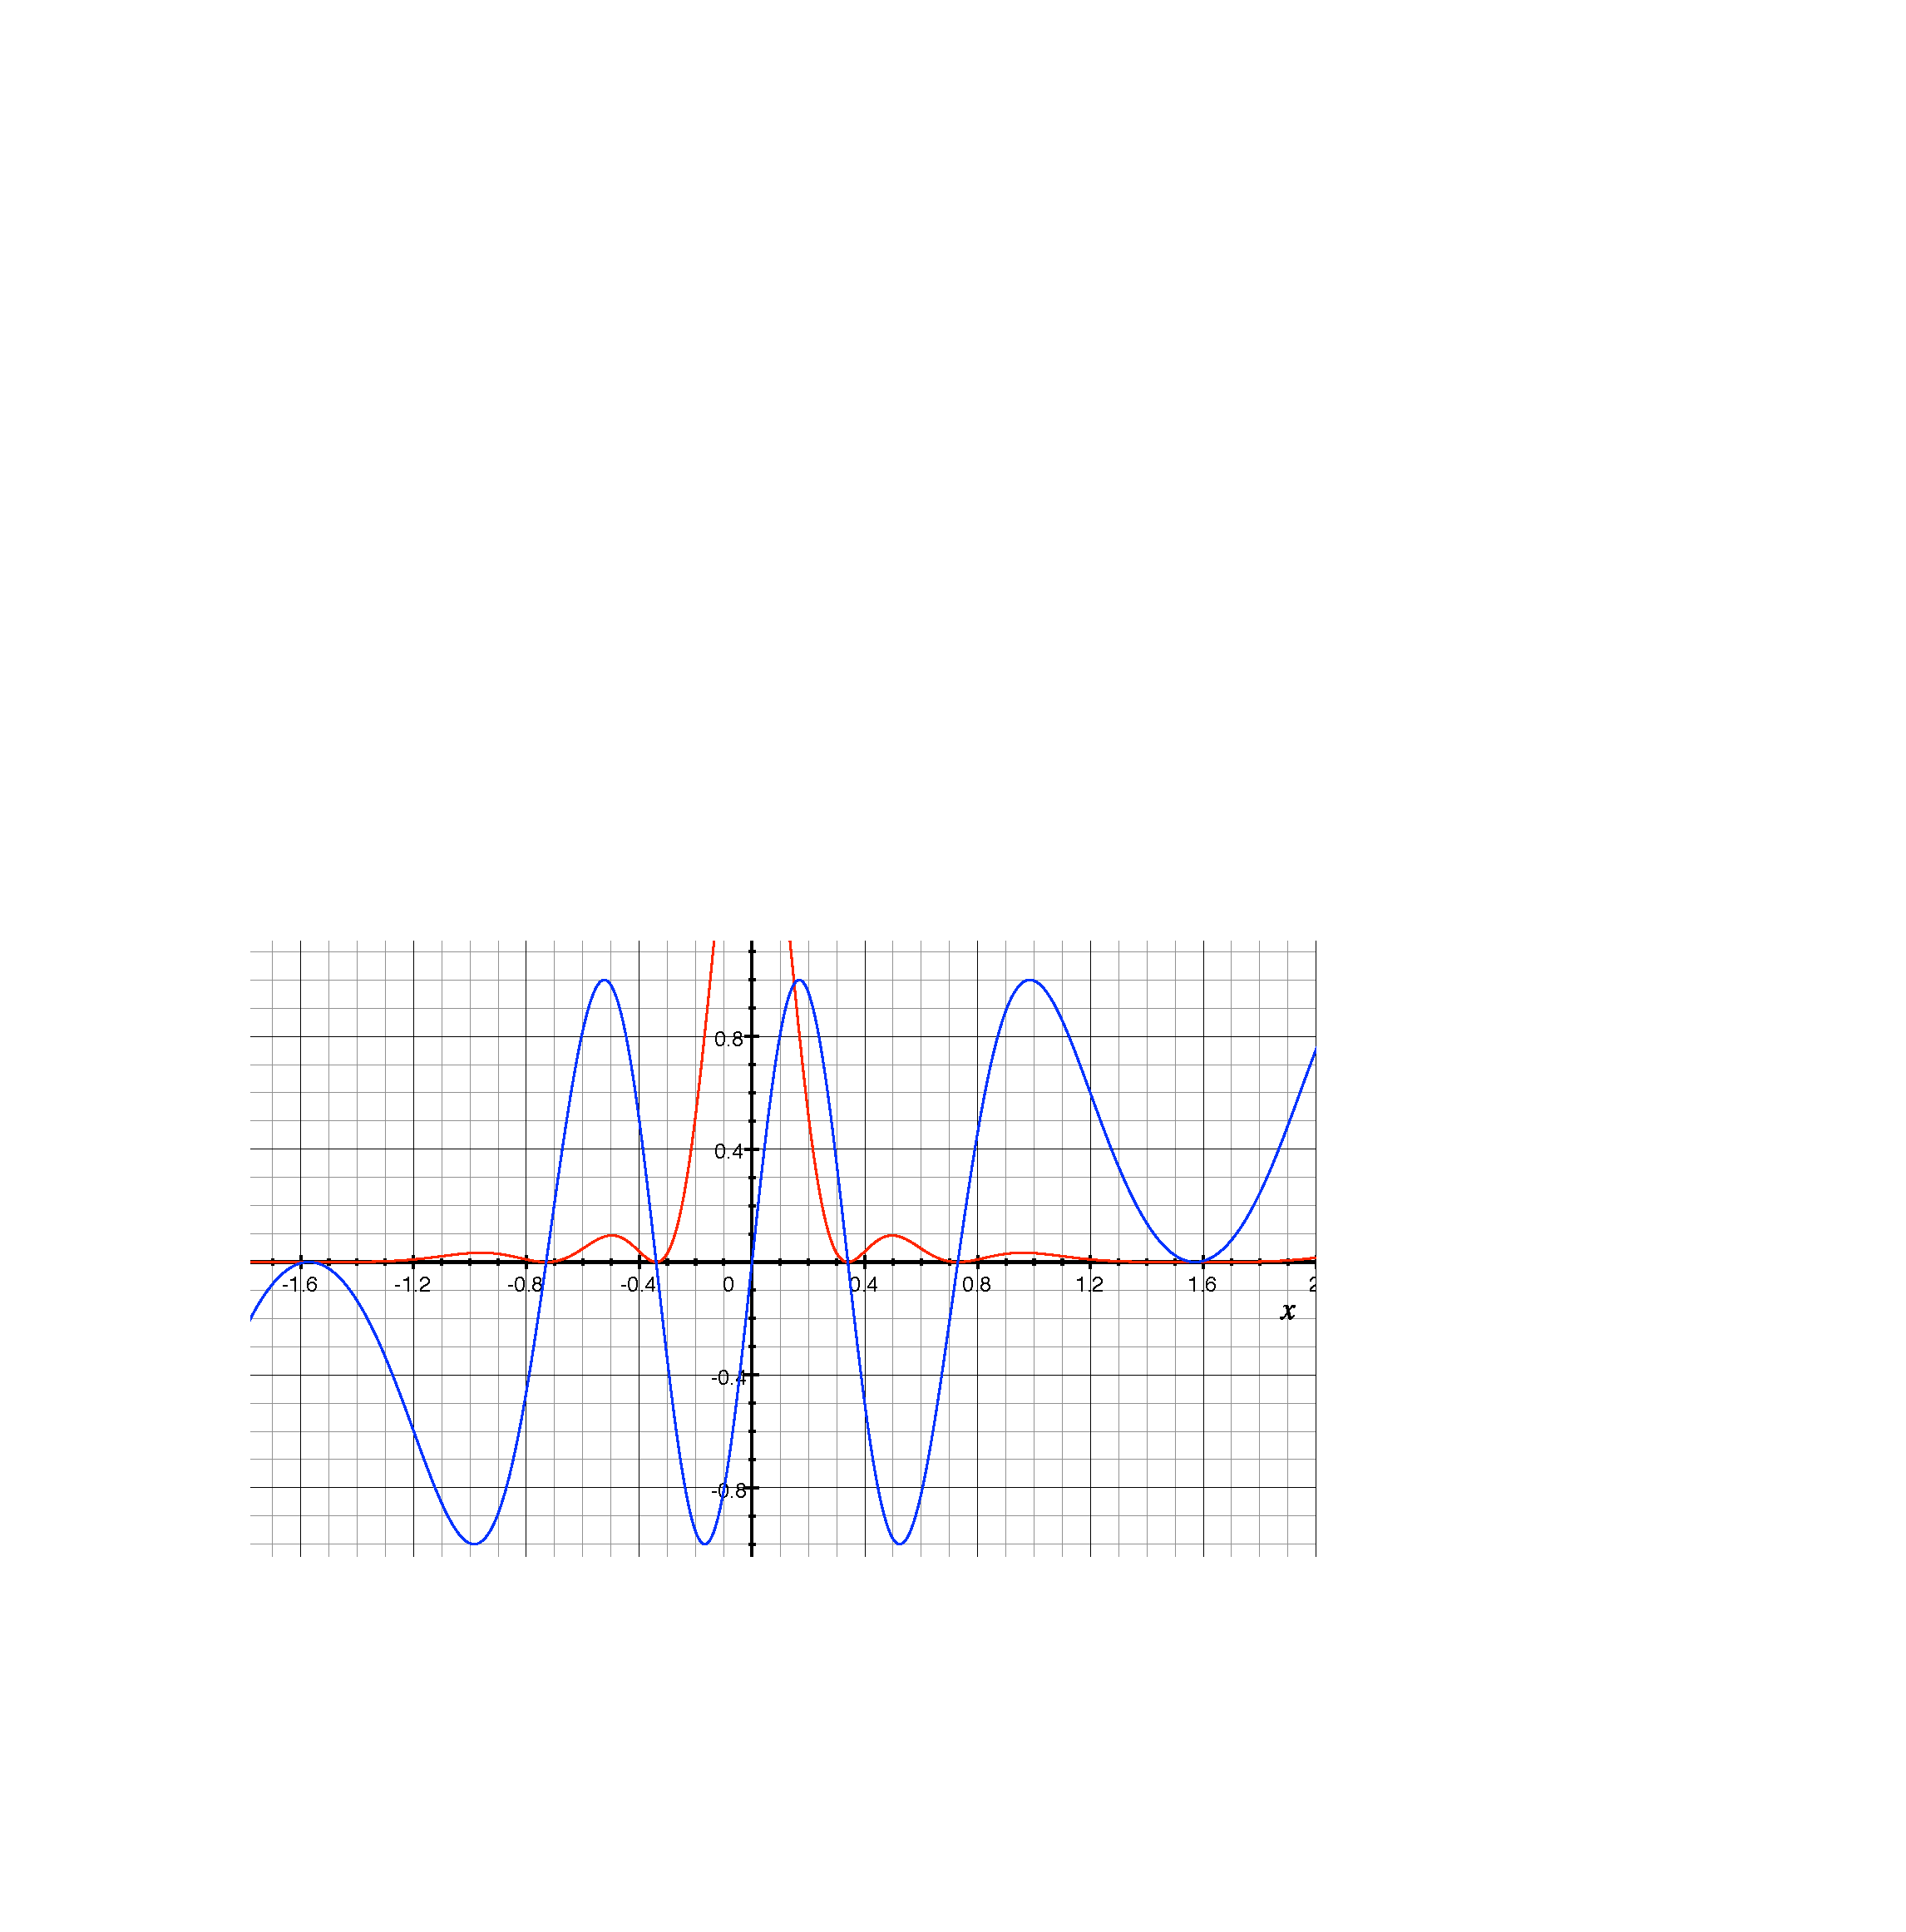
\includegraphics[width=100mm]{resources/minima.pdf}
 \caption{Minima van het intensiteitspatroon.}
  \label{fig:minima}
\end{center}
\end{figure}

We merken op dat indien $n = 0$ ook $\theta = 0$ kan zijn. In dit geval zal de sinus-factor tevens een nulpunt-opleveren dat een maximum oplevert, het extremum.

We hebben nu de minima gevonden via de eerste twee factoren. De derde factor moet dus de nulpunten opleveren die leiden tot de maxima. We  kunnen deze schrijven als
\begin{equation} \label{eq:maxima}
r \pi \ \sin \theta \ . \ \cos( r \pi \ \sin \theta) = \sin( r \pi \ \sin \theta)
\end{equation}
of
\begin{equation} \label{eq:maxima2}
r \pi \ \sin \theta = \frac{\sin( r \pi \ \sin \theta)}{\cos( r \pi \ \sin \theta)} = \tan(r \pi \ \sin \theta)
\end{equation}
of
\begin{equation} \label{eq:maxima3}
tan(r \pi \ \sin \theta) - r \pi \ \sin \theta = 0
\end{equation}
wat samen met vergelijking (\ref{eq:alpha-simple}) de niet-lineaire vergelijking (\ref{eq:non-linear}) oplevert. Ook $\theta = 0$ is een nulpunt van deze vergelijking, waardoor ze zeker alle nulpunten oplevert voor de maxima.

\section{Analyse van de substitutiemethodes}

We bekijken vier verschillende substitutiemethodes om de wortels te berekenen van vergelijking (\ref{eq:non-linear}). De nulpunten die we willen vinden zijn $0, \pm4.49340$ en $\pm7.72525$. We beperken ons verder tot de positieve nulpunten omwille van symmetrie. Ingevuld in vergelijking (\ref{eq:alpha-simple}) levert ons dat voor het voorbeeld met $r=3$ waarden voor $\theta$: 0, 0.49697 en 0.96084. Dit wordt bevestigd door figuur \ref{fig:maxima} waar we zien dat de maxima zich inderdaad voordoen bij deze waarden.

\subsection{$F(x) = \tan(x)$}

Wanneer we de tangens functie gebruiken in de substitutiemethode, merken we dat deze alleen convergeert naar het nulpunt met waarde nul. Dit is niet verwonderlijk, aangezien we weten dat convergentie alleen zal optreden bij een vast punt $x^*$ van $F(x)$ als $|F'(x^*)| < 1$. Voor de verwachte vaste punten 4,49340 en 7,72525 levert $|F'(x^*)|$ respectievelijk 21.18892 en 60.67779 op. Alleen voor nul bekomen we nog juist de waarde 1.

\subsection{$F(x,k) = \arctan(x) + k\pi$}

De geparameteriseerde functie op basis van de boogtangens levert op zeer eenvoudige wijze alle gezochte nulpunten. Wanneer we $k \in \mathbb{N}$ nemen, krijgen we de opeenvolgende nulpunten. Hierbij kunnen we eenvoudig telkens dezelfde startwaarde (b.v.b.\ 1) nemen. Figuur \ref{fig:arctan} toont de situatie voor het eerste nulpunt dat van nul verschilt.

\begin{figure}
\begin{center}
 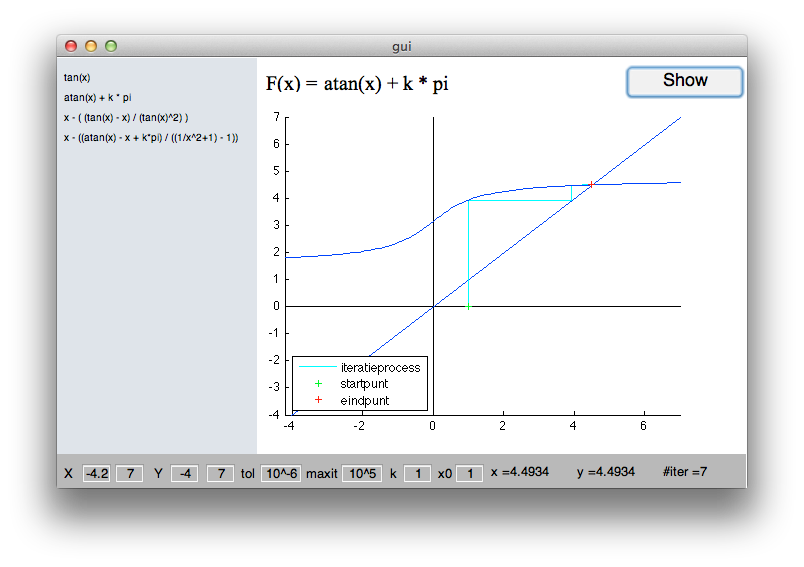
\includegraphics[width=120mm]{resources/arctan.png}
 \caption{Benadering van een nulpunt met $F(x,k) = \arctan(x) + k\pi$ met $k=1$}
  \label{fig:arctan}
\end{center}
\end{figure}

\subsection{Newton-Raphson voor $f(x) = \tan(x) - x$}

Wanneer we $\tan(x) - x$ toepassen met Newton-Raphson en de substitutieformule $x - \frac{tan(x) - x}{tan(x)^2}$ toepassen, merken we dat we opnieuw redelijk eenvoudig het nulpunt voor het extremum vinden. Ook de overige nulpunten zijn te benaderen. Hier moeten we echter een startwaarde kiezen die reeds zeer dicht bij het gezochte nulpunt ligt. Zo moeten we b.v.b.\ om het nulpunt 4,49340 te vinden minstens 4,3 als startwaarde gebruiken.

\subsection{Newton-Raphson voor $f(x) = \arctan(x) - x + k\pi$}

Net zoals bij de eerste functie, merken we opnieuw dat de voorwaarde voor convergentie alleen mogelijk is voor het nulpunt met waarde nul. De parameter $k$ stelt ons in staat om deze hellingsgraad te be\"invloeden, echter nooit tot een bruikbare situatie. Potenti\"ele nulpunten, in de vorm van snijpunten tussen de functie $x - \frac{\arctan(x) - x + k*pi}{\frac{1}{x^2+1} - 1}$ en de $1^e$ bissectrice ontbreken sowieso. Opnieuw zouden we dit wel kunnen cre\"eren door goede waardes voor $k$ te kiezen, alleen zou nog steeds een perfect startpunt nodig zijn om divergentie vermijden.

\subsection{Convergentiegedrag en nauwkeurigheid}

Aangezien alleen de tweede functie ($\arctan(x) + k\pi$) in staat is om meerdere nulpunten te benaderen, bekijken we het convergentiegedrag voor deze functie. Figuur \ref{fig:convergentie-error} toont de relatieve fout bij opeenvolgende iteraties.

\begin{figure}
\begin{center}
 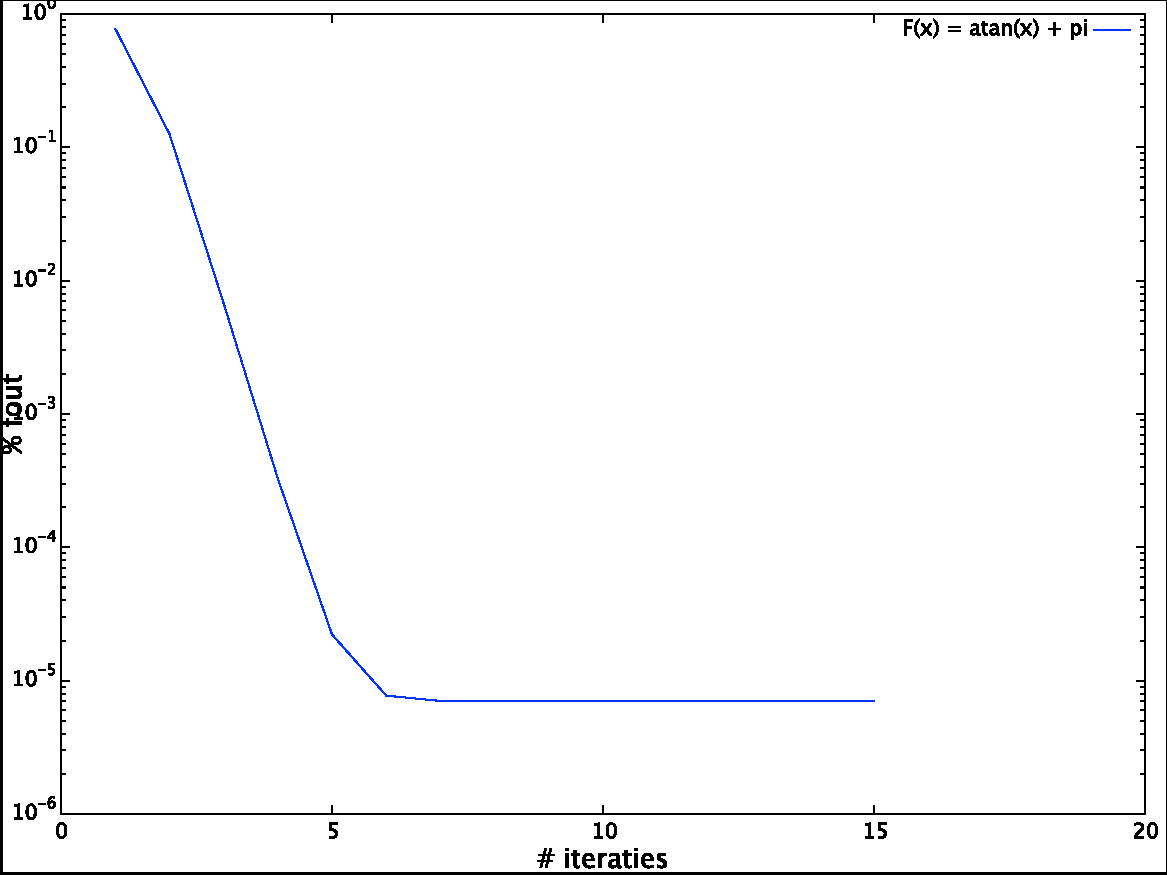
\includegraphics[width=80mm]{resources/convergentie-error.pdf}
 \caption{Relatieve fout in functie van het aantal iteraties}
  \label{fig:convergentie-error}
\end{center}
\end{figure}

Aan de hand van de parameters \emph{tol} en \emph{maxit} kan de precisie van het resultaat verhoogd worden. Door afwisselend beide, indien mogelijk/nodig, te verhogen kunnen we op zoek gaan naar een resultaat dat niet meer wijzigt. In het geval van de tweede functie zien we dat deze nooit meer dan 14 iteraties nodig heeft om het eerste nulpunt te vinden. Hierbij kan de tolerantie verlaagd worden tot $10^{-16}$, waarna zowel het resultaat als het aantal iteraties niet meer wijzigen. Vanaf een tolerantie van $10^{-14}$ wordt reeds het finale resultaat bereikt.

De gevonden waarde is 4,493409457909064, waar de verwachte waarde 4,493440945790906 is, of een absolute fout van $-3.148788184148543 10^{-05}$ of een nauwkeurigheid tot op 4 cijfers na de komma.

\section{Tijdsbesteding}

\begin{longtable}{l|r}
 Totaal in uren& 29.75 \\
 \hline
\endfirsthead
 & 29.75 \\
\endhead
\multicolumn{2}{r}{{Continued\ldots}} \
\endfoot
\hline
\endlastfoot

Schrijven code GUI & 9.25 \\
Theoretische analyse van de verschillende substitutiemethodes & 10.00 \\
Schrijven code overige functies & 3.50 \\
Debuggen & 1.00 \\
Schrijven verslag & 6.00 \\

\end{longtable}

\end{document}
